\documentclass[11pt]{article}
%%%%%%%%% options for the file macros.tex

\def\showauthornotes{1}
\def\showkeys{0}
\def\showdraftbox{0}
% \allowdisplaybreaks[1]

%% Shamelessly adapted from a scribe template by Sanjeev Arora

%%%%%%%%%%%%%% Packages
% \usepackage[active,tightpage]{preview}
% \renewcommand{\PreviewBorder}{1in}
\usepackage[hidelinks]{hyperref}
\usepackage{amsmath,amssymb,amsthm,amstext,amsfonts,bbm,algorithm,algorithmicx,xspace,nicefrac,
  algpseudocode}
\usepackage{color,stmaryrd,enumerate,latexsym,bm,amsfonts,
  subfigure,wrapfig,verbatim,tabularx,textcomp}
\usepackage[small]{caption}
\usepackage{comment} 
\usepackage{epsfig} 
\usepackage{latexsym,nicefrac,bbm}
\usepackage{xspace}
\usepackage{color,fancybox,graphicx,url,subfigure}
\usepackage{enumitem, fullpage}
\usepackage{booktabs}
\usepackage{commath}
\usepackage{mdframed}
\usepackage{pdfsync}
\usepackage{tikz}
\usetikzlibrary {positioning}

%%%%%%%%%%%%%% Use for definitions
\newcommand{\defeq}{\stackrel{\textup{def}}{=}}

\DeclareMathOperator*{\argmax}{arg\,max}
\DeclareMathOperator*{\argmin}{arg\,min}

%%%%%%%%%%%%%% Theorem Environments
\newtheorem{theorem}{Theorem}[section]
\newtheorem{problem}[theorem]{Problem}
\newtheorem{lemma}[theorem]{Lemma}
\newtheorem{definition}[theorem]{Definition}
\newtheorem{corollary}[theorem]{Corollary}
\newtheorem{conjecture}[theorem]{Conjecture}
\newtheorem{proposition}[theorem]{Proposition}
\newtheorem{fact}[theorem]{Fact}
\newtheorem{remark}[theorem]{Remark}

%%%%%%%%%%%%%% Probability stuff
\DeclareMathOperator*{\pr}{\bf Pr}
\DeclareMathOperator*{\av}{\mathbbm{E}}
\DeclareMathOperator*{\var}{\bf Var}

%%%%%%%%%%%%%% Matrix stuff
\newcommand{\tr}[1]{\mathop{\mbox{Tr}}\left({#1}\right)}
\newcommand{\diag}[1]{{\bf Diag}\left({#1}\right)}

%% Notation for integers, natural numbers, reals, fractions, sets, cardinalities
%%and so on
\newcommand{\nfrac}[2]{\nicefrac{#1}{#2}}
\def\abs#1{\left| #1 \right|}
\renewcommand{\norm}[1]{\ensuremath{\left\lVert #1 \right\rVert}}

\newcommand{\floor}[1]{\left\lfloor\, {#1}\,\right\rfloor}
\newcommand{\ceil}[1]{\left\lceil\, {#1}\,\right\rceil}

\newcommand{\pair}[1]{\left\langle{#1}\right\rangle} %for inner product

\newcommand\B{\{0,1\}}      % boolean alphabet  use in math mode
\newcommand\bz{\mathbb Z}
\newcommand\nat{\mathbb N}
\newcommand\rea{\mathbb R}
\newcommand\com{\mathbb{C}}
\newcommand\plusminus{\{\pm 1\}}
\newcommand\Bs{\{0,1\}^*}   % B star use in math mode
\newcommand{\ones}{\mathbbm{1}}
\newcommand{\eye}{\mathbbm{I}}



\newcommand{\V}[1]{\mathbf{#1}\ignorespaces}
\renewcommand\AA{\boldsymbol{\mathit{A}}}
\newcommand\LL{\boldsymbol{\mathit{L}}}

% Used to denote bold commands
                                % e.g. vectors, matrices
\DeclareRobustCommand{\fracp}[2]{{#1 \overwithdelims()#2}}
\DeclareRobustCommand{\fracb}[2]{{#1 \overwithdelims[]#2}}
\newcommand{\marginlabel}[1]%
{\mbox{}\marginpar{\it{\raggedleft\hspace{0pt}#1}}}
\newcommand\card[1]{\left| #1 \right|} %cardinality of set S; usage \card{S}
\renewcommand\set[1]{\left\{#1\right\}} %usage \set{1,2,3,,}
\renewcommand\complement{\ensuremath{\mathsf{c}}}
\newcommand\poly{\mbox{poly}}  %usage \poly(n)
\newcommand{\comp}[1]{\overline{#1}}
\newcommand{\smallpair}[1]{\langle{#1}\rangle}
\newcommand{\ol}[1]{\ensuremath{\overline{#1}}\xspace}
\newcommand{\eps}{\epsilon}
\DeclareMathOperator{\vol}{\mathsf{vol}}


%%%%%%%%%%%%%% Mathcal shortcuts
\newcommand\calF{\mathcal{F}}
\newcommand\calP{\mathcal{P}}
\newcommand\calS{\mathcal{S}}
\newcommand\calG{\mathcal{G}}
\newcommand\calH{\mathcal{H}}
\newcommand\calC{\mathcal{C}}
\newcommand\calD{\mathcal{D}}
\newcommand\calI{\mathcal{I}}
\newcommand\calV{\mathcal{V}}
\newcommand\calK{\mathcal{K}}
\newcommand\calN{\mathcal{N}}
\newcommand\calX{\mathcal{X}}
\newcommand\calU{\mathcal{U}}
\newcommand\calE{\mathcal{E}}
\newcommand\calL{\mathcal{L}}
\newcommand\calR{\mathcal{R}}


%%%%%%%%%%%%%% {{{ authornotes }}}
\definecolor{Mygray}{gray}{0.8}

 \ifcsname ifcommentflag\endcsname\else
  \expandafter\let\csname ifcommentflag\expandafter\endcsname
                  \csname iffalse\endcsname
\fi

\ifnum\showauthornotes=1
\newcommand{\todo}[1]{\colorbox{Mygray}{\color{red}#1}}
\else
\newcommand{\todo}[1]{#1}
\fi

\ifnum\showauthornotes=1
\newcommand{\Authornote}[2]{{\sf\small\color{red}{[#1: #2]}}}
\newcommand{\Authoredit}[2]{{\sf\small\color{red}{[#1]}\color{blue}{#2}}}
\newcommand{\Authorcomment}[2]{{\sf \small\color{gray}{[#1: #2]}}}
\newcommand{\Authorfnote}[2]{\footnote{\color{red}{#1: #2}}}
\newcommand{\Authorfixme}[1]{\Authornote{#1}{\textbf{??}}}
\newcommand{\Authormarginmark}[1]{\marginpar{\textcolor{red}{\fbox{%\Large
#1:!}}}}
\else
\newcommand{\Authornote}[2]{}
\newcommand{\Authoredit}[2]{}
\newcommand{\Authorcomment}[2]{}
\newcommand{\Authorfnote}[2]{}
\newcommand{\Authorfixme}[1]{}
\newcommand{\Authormarginmark}[1]{}
\fi


%%%%%%%%%%%%%% Logical operators
\newcommand\true{\mbox{\sc True}}
\newcommand\false{\mbox{\sc False}}
\def\scand{\mbox{\sc and}}
\def\scor{\mbox{\sc or}}
\def\scnot{\mbox{\sc not}}
\def\scyes{\mbox{\sc yes}}
\def\scno{\mbox{\sc no}}

%% Parantheses
\newcommand{\paren}[1]{\unskip\left({#1}\right)}
\newcommand{\sqparen}[1]{\unskip\left[{#1}\right]}
\newcommand{\curlyparen}[1]{\unskip\left\{{#1}\right\}}
\newcommand{\smallparen}[1]{\unskip({#1})}
\newcommand{\smallsqparen}[1]{\unskip[{#1}]}
\newcommand{\smallcurlyparen}[1]{\unskip\{{#1}\}}

%% short-hands for relational simbols

\newcommand{\from}{:}
\newcommand\xor{\oplus}
\newcommand\bigxor{\bigoplus}
\newcommand{\logred}{\leq_{\log}}
\def\iff{\Leftrightarrow}
\def\implies{\Rightarrow}

%--------------------------------------------------------------------------------------------------------------------------------
% Optimization macros
%--------------------------------------------------------------------------------------------------------------------------------
%\providecommand{\argmax}{\mathop\mathrm{arg max}} % Defining math symbols
%\providecommand{\argmin}{\mathop\mathrm{arg min}}
\providecommand{\arccos}{\mathop\mathrm{arccos}}
\providecommand{\dom}{\mathop\mathrm{dom}}
\providecommand{\diag}{\mathop\mathrm{diag}}
\providecommand{\tr}{\mathop\mathrm{tr}}
%\providecommand{\abs}{\mathop\mathrm{abs}}
\providecommand{\card}{\mathop\mathrm{card}}
\providecommand{\sign}{\mathop\mathrm{sign}}
\providecommand{\conv}{\mathop\mathrm{conv}} % Convex hull
\def\rank#1{\mathrm{rank}({#1})}
\def\supp#1{\mathrm{supp}({#1})}

\providecommand{\minimize}{\mathop\mathrm{minimize}}
\providecommand{\maximize}{\mathop\mathrm{maximize}}
\providecommand{\subjectto}{\mathop\mathrm{subject\;to}}

%\renewcommand\eqref[1]{Eq.~(\ref{#1})}

\def\openright#1#2{\left[{#1}, {#2}\right)}

%--------------------------------------------------------------------------------------------------------------------------------
% Vectors and matrices
%--------------------------------------------------------------------------------------------------------------------------------
\newcommand{\boldone}{\mbf{1}} % Bold 1
\newcommand{\ident}{\mbf{I}} % Identity matrix
% \def\v#1{\mbi{#1}} % Vector notation
%\def\norm#1{\left\|{#1}\right\|} % A norm with 1 argument
\newcommand{\onenorm}[1]{\norm{#1}_1} % L1 norm
\newcommand{\twonorm}[1]{\norm{#1}_2} % L2 norm
\newcommand{\infnorm}[1]{\norm{#1}_{\infty}} % Linfty norm
\newcommand{\opnorm}[1]{\norm{#1}_{\text{op}}} % Operator norm
\newcommand{\fronorm}[1]{\norm{#1}_{\text{F}}} % Frobenius norm
\newcommand{\nucnorm}[1]{\norm{#1}_{*}} % Frobenius norm
\def\staticnorm#1{\|{#1}\|} % A static norm that does not resize with input
\newcommand{\statictwonorm}[1]{\staticnorm{#1}_2} % L2 norm
\newcommand{\inner}[1]{{\langle #1 \rangle}} % inner product
\newcommand{\binner}[2]{\left\langle{#1},{#2}\right\rangle} % Inner product with expandable brackets
\def\what#1{\widehat{#1}}

\def\twovec#1#2{\left[\begin{array}{c}{#1} \\ {#2}\end{array}\right]}
\def\threevec#1#2#3{\left[\begin{array}{c}{#1} \\ {#2} \\ {#3} \end{array}\right]}
\def\nvec#1#2#3{\left[\begin{array}{c}{#1} \\ {#2} \\ \vdots \\ {#3}\end{array}\right]} % An n-vector with three arguments
\DeclareMathOperator\spn{span}


%% macros to write pseudo-code

\newlength{\pgmtab}  %  \pgmtab is the width of each tab in the
\setlength{\pgmtab}{1em}  %  program environment
 \newenvironment{program}{\renewcommand{\baselinestretch}{1}%
\begin{tabbing}\hspace{0em}\=\hspace{0em}\=%
\hspace{\pgmtab}\=\hspace{\pgmtab}\=\hspace{\pgmtab}\=\hspace{\pgmtab}\=%
\hspace{\pgmtab}\=\hspace{\pgmtab}\=\hspace{\pgmtab}\=\hspace{\pgmtab}\=%
\+\+\kill}{\end{tabbing}\renewcommand{\baselinestretch}{\intl}}
\newcommand {\BEGIN}{{\bf begin\ }}
\newcommand {\ELSE}{{\bf else\ }}
\newcommand {\IF}{{\bf if\ }}
\newcommand {\FOR}{{\bf for\ }}
\newcommand {\TO}{{\bf to\ }}
\newcommand {\DO}{{\bf do\ }}
\newcommand {\WHILE}{{\bf while\ }}
\newcommand {\ACCEPT}{{\bf accept}}
\newcommand {\REJECT}{\mbox{\bf reject}}
\newcommand {\THEN}{\mbox{\bf then\ }}
\newcommand {\END}{{\bf end}}
\newcommand {\RETURN}{\mbox{\bf return\ }}
\newcommand {\HALT}{\mbox{\bf halt}}
\newcommand {\REPEAT}{\mbox{\bf repeat\ }}
\newcommand {\UNTIL}{\mbox{\bf until\ }}
\newcommand {\TRUE}{\mbox{\bf true\ }}
\newcommand {\FALSE}{\mbox{\bf false\ }}
\newcommand {\FORALL}{\mbox{\bf for all\ }}
\newcommand {\DOWNTO}{\mbox{\bf down to\ }}

% Theorem-type environments
% \theoremstyle{break} 
% \theoremheaderfont{\scshape}
% \theorembodyfont{\slshape}
% \newtheorem{Thm}{Theorem}[section]
% \newtheorem{Lem}[Thm]{Lemma}
% \newtheorem{Cor}[Thm]{Corollary}
% \newtheorem{Prop}[Thm]{Proposition}
% % \theoremstyle{plain} 
% % \theorembodyfont{\rmfamily} 
% \newtheorem{Ex}[Thm]{Exercise}
% \newtheorem{Exa}[Thm]{Example}
% \newtheorem{Rem}[Thm]{Remark}
% % \theorembodyfont{\itshape}
% \newtheorem{Def}[Thm]{Definition}
% \newtheorem{Conj}[Thm]{Conjecture}
% \newtheorem{Obs}[Thm]{Observation}
% \newtheorem{Ques}[Thm]{Question}
%\newenvironment{proof}{\noindent {\sc Proof:}}{$\Box$ \medskip} 
\newenvironment{problems} % Definition of problems
 {\renewcommand{\labelenumi}{\S\theenumi}
	\begin{enumerate}}{\end{enumerate}}


%%%%%%%%%%%%%%%%% Proof Environments

\def\FullBox{\hbox{\vrule width 6pt height 6pt depth 0pt}}
%
%\def\qed{\ifmmode\qquad\FullBox\else{\unskip\nobreak\hfil
%\penalty50\hskip1em\null\nobreak\hfil\FullBox
%\parfillskip=0pt\finalhyphendemerits=0\endgraf}\fi}

\def\qedsketch{\ifmmode\Box\else{\unskip\nobreak\hfil
\penalty50\hskip1em\null\nobreak\hfil$\Box$
\parfillskip=0pt\finalhyphendemerits=0\endgraf}\fi}

%\newenvironment{proof}{\begin{trivlist} \item {\bf Proof:~~}}
 %  {\qed\end{trivlist}}

\newenvironment{proofsketch}{\begin{trivlist} \item {\bf
Proof Sketch:~~}}
  {\qedsketch\end{trivlist}}

\newenvironment{proofof}[1]{\begin{trivlist} \item {\bf Proof
#1:~~}}
  {\qed\end{trivlist}}

\newenvironment{claimproof}{\begin{quotation} \noindent
{\bf Proof of claim:~~}}{\qedsketch\end{quotation}}


%%%%%%%%%%%%%%%%%%%%%%%%%%%%%%%%%%%%%%%%%%%%%%%%%%%%%%%%%%%%%%%%%%%%%%%%%%%
%%%%%%%%%%%%%%%%%%%%%%%%%%%%%%%%%%%%%%%%%%%%%%%%%%%%%%%%%%%%%%%%%%%%%%%%%%%




\newlength{\tpush}
\setlength{\tpush}{2\headheight}
\addtolength{\tpush}{\headsep}

\newcommand{\handout}[5]{
   \noindent
   \begin{center}
   \framebox{ \vbox{ \hbox to \textwidth { {\bf \coursenum\ :\  \coursename} \hfill #5 }
       \vspace{3mm}
       \hbox to \textwidth { {\Large \hfill #2  \hfill} }
       \vspace{1mm}
       \hbox to \textwidth { {\it #3 \hfill #4} }
     }
   }
   \end{center}
   \vspace*{4mm}
   \newcommand{\lecturenum}{#1}
   \addcontentsline{toc}{chapter}{Lecture #1 -- #2}
}

\newcommand{\lecturetitle}[4]{\handout{#1}{#2}{Lecturer: \courseprof
  }{Scribes: #3}{Date: #4}}
\newcommand{\guestlecturetitle}[5]{\handout{#1}{#2}{Lecturer:
    #4}{Scribe: #3}{Lecture #1 - #5}}


%%%%%%%%%%%%%%%%%%%%%%%%%%%%%%%%%%%%%%%%%%%%%%%%%%%%%%%%%
%%% Commands to include figures


%% PSfigure

\newcommand{\PSfigure}[3]{\begin{figure}[t] 
  \centerline{\vbox to #2 {\vfil \psfig{figure=#1.eps,height=#2} }} 
  \caption{#3}\label{#1} 
  \end{figure}} 
\newcommand{\twoPSfigures}[5]{\begin{figure*}[t]
  \centerline{%
    \hfil
    \begin{tabular}{c}
        \vbox to #3 {\vfil\psfig{figure=#1.eps,height=#3}} \\ (a)
    \end{tabular}
    \hfil\hfil\hfil
    \begin{tabular}{c}
        \vbox to #3 {\vfil\psfig{figure=#2.eps,height=#3}} \\ (b)
    \end{tabular}
    \hfil}
  \caption{#4}
  \label{#5}
%  \sublabel{#1}{(a)}
%  \sublabel{#2}{(b)}
  \end{figure*}}

\newcounter{fignum}

% fig
%command to insert figure. usage \fig{name}{h}{caption}
%where name.eps is the postscript file and h is the height in inches
%The figure is can be referred to using \ref{name}
\newcommand{\fig}[3]{%
\begin{minipage}{\textwidth}
\centering\epsfig{file=#1.eps,height=#2}
\caption{#3} \label{#1}
\end{minipage}
}%


% ffigure
% Usage: \ffigure{name of file}{height}{caption}{label}
\newcommand{\ffigure}[4]{\begin{figure} 
  \centerline{\vbox to #2 {\hfil \psfig{figure=#1.eps,height=#2} }} 
  \caption{#3}\label{#4} 
  \end{figure}} 

% ffigureh
% Usage: \ffigureh{name of file}{height}{caption}{label}
\newcommand{\ffigureh}[4]{\begin{figure}[!h] 
  \centerline{\vbox to #2 {\vfil \psfig{figure=#1.eps,height=#2} }} 
  \caption{#3}\label{#4} 
  \end{figure}} 


% {{{ draftbox }}}
\ifnum\showdraftbox=1
\newcommand{\draftbox}{\begin{center}
  \fbox{%
    \begin{minipage}{2in}%
      \begin{center}%
%        \begin{Large}%
          \large\textsc{Working Draft}\\%
%        \end{Large}\\
        Please do not distribute%
      \end{center}%
    \end{minipage}%
  }%
\end{center}
\vspace{0.2cm}}
\else
\newcommand{\draftbox}{}
\fi


%% Complexity classes
\newcommand\p{\mbox{\bf P}\xspace}
\newcommand\np{\mbox{\bf NP}\xspace}
\newcommand\cnp{\mbox{\bf coNP}\xspace}
\newcommand\sigmatwo{\mbox{\bf $\Sigma_2$}\xspace}
\newcommand\ppoly{\mbox{\bf $\p_{\bf /poly}$}\xspace}
\newcommand\sigmathree{\mbox{\bf $\Sigma_3$}\xspace}
\newcommand\pitwo{\mbox{\bf $\Pi_2$}\xspace}
\newcommand\rp{\mbox{\bf RP}\xspace}
\newcommand\zpp{\mbox{\bf ZPP}\xspace}
\newcommand\bpp{\mbox{\bf BPP}\xspace}
\newcommand\ph{\mbox{\bf PH}\xspace}
\newcommand\pspace{\mbox{\bf PSPACE}\xspace}
\newcommand\npspace{\mbox{\bf NPSPACE}\xspace}
\newcommand\dl{\mbox{\bf L}\xspace}
\newcommand\ma{\mbox{\bf MA}\xspace}
\newcommand\am{\mbox{\bf AM}\xspace}
\newcommand\nl{\mbox{\bf NL}\xspace}
\newcommand\conl{\mbox{\bf coNL}\xspace}
\newcommand\sharpp{\mbox{\#{\bf P}}\xspace}
\newcommand\parityp{\mbox{$\oplus$ {\bf P}}\xspace}
\newcommand\ip{\mbox{\bf IP}\xspace}
\newcommand\pcp{\mbox{\bf PCP}}
\newcommand\dtime{\mbox{\bf DTIME}}
\newcommand\ntime{\mbox{\bf NTIME}}
\newcommand\dspace{\mbox{\bf SPACE}\xspace}
\newcommand\nspace{\mbox{\bf NSPACE}\xspace}
\newcommand\cnspace{\mbox{\bf coNSPACE}\xspace}
\newcommand\exptime{\mbox{\bf EXP}\xspace}
\newcommand\nexptime{\mbox{\bf NEXP}\xspace}
\newcommand\genclass{\mbox{$\cal C$}\xspace}
\newcommand\cogenclass{\mbox{\bf co$\cal C$}\xspace}
\newcommand\size{\mbox{\bf SIZE}\xspace}
\newcommand\sig{\mathbf \Sigma}
\newcommand\pip{\mathbf \Pi}

%%Computational problems
\newcommand\sat{\mbox{SAT}\xspace}
\newcommand\tsat{\mbox{3SAT}\xspace}
\newcommand\tqbf{\mbox{TQBF}\xspace}
\def\E{\mathbb{E}}
\newcommand{\vone}{\boldsymbol{\mathbf{1}}}
\allowdisplaybreaks

\usepackage{tikz}
\usepackage{amsmath, amsfonts, amsthm, amssymb, mathtools, mathrsfs}

\usepackage[
    backend=biber,
% giveninits=true,
% natbib=true,
    style=alphabetic,
    url=false, 
 %   doi=true,
    hyperref,
    backref=true,
    backrefstyle=none,
    maxbibnames=10,
    sortcites
]{biblatex}
\addbibresource{papers.bib}

%%%%%%%%% Authornotes
\newcommand{\Snote}{\Authornote{S}}

\newenvironment{tight_enumerate}{
\begin{enumerate}
 \setlength{\itemsep}{2pt}
 \setlength{\parskip}{1pt}
}{\end{enumerate}}
\newenvironment{tight_itemize}{
\begin{itemize}
 \setlength{\itemsep}{2pt}
 \setlength{\parskip}{1pt}
}{\end{itemize}}



\addbibresource{refs.bib}

%%%%%%%%%%%%%%%%%%%%%%%%%

\begin{document}

\newcommand{\coursenum}{{CSC 2240H}}
\newcommand{\coursename}{{Graphs, Matrices, and Optimization}}
\newcommand{\courseprof}{Sushant Sachdeva}

\lecturetitle{1}{Higher Order Cheeger's Inequalities}{Amirmojtaba Sabour, Alireza Mousavi-Hosseini}{23 Dec 2022}

\section{Introduction}
Recall that given a weighted undirected graph $G = (V, E, w)$ and a subset of vertices $S \subset V$, the conductance of $S$ is defined as
\begin{equation}
    \phi(S) \coloneqq \frac{\sum_{u \in S, v \in \overline{S}} w(u, v)}{\min(\vol(S),\vol(\overline{S}))}
\end{equation}
where $\vol(S) \coloneqq \sum_{v \in S} w(v)$.
The conductance of the graph is defined as the minimum conductance over all cuts 
\begin{equation}
    \phi(G) \coloneqq \min_{S \subset G} \phi(S).
\end{equation}
The Laplacian is defined as $L \coloneqq D - A$ and the Normalized Laplacian is defined as $\calL \coloneqq I - D^{-1/2}AD^{-1/2}$. Finally, let $0 = \lambda_1 \leq \lambda_2 \leq ... \leq \lambda_n \leq 2$ represent the eigenvalues of $\calL$. 

The original Cheeger's inequality states that
\begin{equation}
    \frac{\lambda_2}{2} \leq \phi(G) \leq \sqrt{2\lambda_2}.
\end{equation}
In this lecture, we look at improving the upper bound by utilizing higher order eigenvalues. Formally, we will prove the following theorem.
\begin{theorem}\label{thm:improved_cheeger}
    For every undirected graph $G$ and every $k \geq 2$,
    \begin{equation}\label{eq:improved_cheeger}
    \phi(G) = O(k) \frac{\lambda_2}{\sqrt{\lambda_k}}.
\end{equation}
\end{theorem}
This inequality is sharp in general as it can be shown that on the circle graph $\phi(G) = \Omega(k\lambda_2/\sqrt{\lambda_k})$.

In the following, we will begin by introducing several definitions and lemmas that will be central to the argument. Then, we will present the proof of Theorem \ref{thm:improved_cheeger}, which will be divided into three steps. 


\section{Preliminaries}
Given a function $f: V \to \mathbb{R}$, we will introduce several useful definitions. First, we establish a notion of cuts associated to $f$ with different threshold values. Given a threshold $t \in \rea$, we define the threshold set to be  $V_f(t) \coloneqq \{ v \in V \, : \, f(v) \geq t\}$. The conductance of $f$ is then defined to be the minimum of the conductance of its threshold sets, i.e.\ $\phi(f) \coloneqq \min_{t} \phi(V_f(t))$.

For clarity of presentation, we let $\ell^2(V)$ and $\ell^2(V,w)$ be Hilbert spaces of functions $f : V \to \rea$ with the usual dot product (denoted by $\binner{.}{.}$) and $\binner{f}{g}_w = \sum_{v}w(v)f(v)g(v)$ respectively. We also define the $w$-norm as $\norm{f}_w = \sqrt{\binner{f}{f}_w}$. An object that helps us relate properties of $f$ to the eigenspectrum of $\calL$ is the Rayleigh quotient. In this note, we define the Rayleigh quotient of $f$ to be
\begin{equation}
        \calR(f) \coloneqq  \frac{\binner{f}{L f}}{\binner{f}{Df}} = \frac{\binner{D^{\frac{1}{2}} f}{\calL D^{\frac{1}{2}} f}}{\norm{f}_w^2}.
\end{equation}
The precise relationship between the eigenspectrum of $\calL$ and $\calR(f)$ is characterized by the following min-max theorem.
\begin{lemma}\label{lem:minmax}
Let $f_1,...,f_k$ be orthogonal in $\ell^2(V,w)$, then
\begin{equation}
    \lambda_k = \min_{f_1,...,f_k \in \ell^2(V,w)} \max_{f \in \spn(f_1,...f_k)} \calR(f).
\end{equation}
\end{lemma}
Using the above principle, we will prove the following lemma which will be useful for introducing $\lambda_k$ in our analysis.
\begin{lemma} \label{lem1}
    For any $k$ disjointly supported $f_1,...,f_k$,
        $$\lambda_k \leq 2\max_{1\leq i\leq k} \calR(f_i).$$
\end{lemma}
\begin{proof}
Notice that since $f_1,\hdots,f_k$ are disjointly supported, they are orthogonal in $\ell^2(V,w)$. Hence from Lemma \ref{lem:minmax}, it suffices to show for any $h \in \spn(f_1,\hdots,f_k)$ we have $\calR(h) \leq 2\max_i \calR(f_i)$. Let $h = \sum_{i=1}^{k}c_if_i$. Since $f_1,\hdots,f_k$ are disjointly supported, for any $u,v\in V$,
$$\abs{h(u) - h(v)}^2 \leq 2\sum_{i=1}^{k}c_i^2(f_i(u) - f_i(v))^2,$$
where the inequality holds since at most two of the terms in the difference are non-zero. Moreover,
\begin{align*}
    \calR(h) = \frac{\sum_{\{u,v\} \in E}w(u,v)\abs{h(u) - h(v)}^2}{\norm{h}_w^2} &\leq \frac{\sum_{\{u,v\} \in E}\sum_{i=1}^{k}2c_i^2(f_i(u) - f_i(v))^2}{\norm{h}_w^2}\\
    &= \frac{2\sum_{i=1}^{k}c_i^2\sum_{\{u,v\} \in E}w(u,v)(f_i(u) - f_i(v))^2}{\sum_{i=1}^kc_i^2\norm{f_i}_w^2}\\
    &= \frac{2\sum_{i=1}^kc_i^2\norm{f_i}_w^2\calR(f_i)}{\sum_{i=1}^{k}c_i^2\norm{f_i}_w^2} \leq 2\max_{1\leq i\leq k}\calR(f_i).
\end{align*}
\end{proof}
Finally, we introduce the following lemma which allows us to upper bound the conductance of a function when we can compute certain estimates of that function.
\begin{lemma} \label{lem_phi_h}
    For every non-negative $h : V \to \mathbb{R}$ with $\vol(\supp{h}) \leq \vol(V)/2$,
    \begin{equation}
        \phi(h) \leq \frac{\sum_{\{u,v\} \in E}{w(u,v)\abs{h(u) - h(v)}}}{\sum_v w(v)h(v)}\label{eq:phi_h}
    \end{equation}
\end{lemma}
\begin{proof}
We begin by normalizing $h$ such that $\max_v h(v) \leq 1$. Let $t$ be a uniform random variable drawn from $[0,1]$. A simple computation shows that $\E[\vone(v \in V_h(t))] = h(v)$ and assuming $h(v) \geq h(u)$, $\E[\vone(v \in V_h(t))\vone(u \in \overline{V_h(t)})] = h(v) - h(u)$. Furthermore, recall from the Cheeger's inequality lecture notes that for any random variable $t$ and resulting random variables $X_t$ and $Y_t > 0$ we have
$$\min_t \frac{X_t}{Y_t} \leq \frac{\E[X_t]}{\E[Y_t]}.$$
Hence,
$$\min_t \frac{\sum_{v \in V_h(t),u \in \overline{V_h(t)}}w(u,v)}{\sum_{v \in V_h(t)}w(v)} \leq \frac{\E\left[\sum_{v \in V_h(t),u \in \overline{V_h(t)}}w(u,v)\right]}{\E\left[\sum_{v \in V_h(t)}w(v)\right]} = \frac{\sum_{\{u,v\} \in E}w(u,v)\abs{h(u) - h(v)}}{\sum_v w(v)h(v)},$$
Since $\vol(\supp{h}) \leq \vol(V)/2$, the LHS of the first inequality is equal to $\phi(h)$, which completes the proof.
\end{proof}

\section{Proof}

The proof of the theorem is constructive.
We will begin by seeking a ``good" function $f: V \to \mathbb{R}$. 
Next, we will explore the approximation of $f$ using step functions and examine their connection to the higher order eigenvalues of the normalized Laplacian.
Finally, we will show how to upper-bound the conductance of a function $f$ using its step-wise approximation.
Combining all these steps together, we will conclude that the conductance of $f$ satisfies our theorem. Throughout the proof, we will use the notation $\psi_{t_1,\hdots,t_l}(x) = \argmin_{t_i}\abs{x-t_i}$.

\subsection{Constructing a Function $f$}
We start by considering the second eigenvector of the normalized Laplacian. Let $g \in \ell^2(V)$ be the second eigenvector of $\calL$. 
Furthermore, let $g_+(v) \coloneqq \max (g(v), 0)$ and $g_-(v) \coloneqq \min (g(v), 0)$ be the positive and negative components of $g$. 
\begin{proposition}
    Let $f_+ = D^{-\frac{1}{2}}g_+$ and $f_- = -D^{-\frac{1}{2}}g_-$. Then we have the following inequalities:
    \begin{align*}
        \calR(f_+) &\leq \lambda_2 \\
        \calR(f_-) &\leq \lambda_2
    \end{align*}
\end{proposition}

\begin{proof}
    By definition, we have
    \begin{equation*}
        \calR(f_+) = \frac{\binner{D^{\frac{1}{2}} f_+}{\calL D^{\frac{1}{2}} f_+}}{\binner{D^{\frac{1}{2}}f_+}{D^{\frac{1}{2}}f_+}} = \frac{\binner{g_+}{\calL g_+}}{\binner{g_+}{g_+}} = \frac{\binner{g_+}{\calL g_+}}{\norm{g_+}^2}.
    \end{equation*}

    Assuming that $u \in \supp{g_+}$ then
    \begin{align*}
        (\calL g_+)(u) = g_+(u) - \sum_{v: (u, v) \in E} \frac{w(u, v) g_+(v)}{\sqrt{w(u)w(v)}} &= g(u) -  \sum_{v: (u, v) \in E} \frac{w(u, v) g_+(v)}{\sqrt{w(u)w(v)}} \\
        &\leq g(u) -  \sum_{v: (u, v) \in E} \frac{w(u, v) g(v)}{\sqrt{w(u)w(v)}} \\
        &= (\calL g)(u) = \lambda_2 \cdot g(u).
    \end{align*}
    
    Therefore
    \begin{equation*}
        \calR(f_+) = \frac{\binner{g_+}{\calL g_+}}{\norm{g_+}^2} = \frac{\sum_{u \in \supp{g_+}} g_+(u) \cdot (\calL g_+)(u)}{\sum_{u \in \supp{g_+}} g_+(u)^2} \leq 
        \frac{\sum_{u \in \supp{g_+}} \lambda_2 \cdot g_+(u)^2}{\sum_{u \in \supp{g_+}} g_+(u)^2} = \lambda_2.
    \end{equation*}

    Similarly, we can show that $\calR(f_-) \leq \lambda_2$. 
\end{proof}

Therefore $f_+, f_-$ are two disjointly supported non-negative functions such that $\calR(f_+),\calR(f_-) \leq \lambda_2$. Choosing the one with the smallest support volume and normalizing, we obtain the following corollary.
\begin{corollary}\label{cor:good_f}
    There exists $f \in \ell^2(V,w)$ such that
    \begin{enumerate}
        \item $f \geq 0$
        \item $\calR(f) \leq \lambda_2$ 
        \item $\vol(\supp{f}) \leq \frac{\vol(V)}{2}$
        \item $\norm{f}_w = 1$.
    \end{enumerate}
\end{corollary}


\subsection{Approximation with Step Functions and Higher Order Eigenvalues}
\begin{definition}
    Given a function $f \in \ell^2(V,w)$, we say $g \in \ell^2(V,w)$ is an $l$-step approximation of $f$ if there exist $0 = t_0 \leq t_1 \leq  t_2 \leq \dots \leq t_{l-1}$ such that 
    \begin{equation*}
        g(v) = \psi_{t_0, t_1, t_2, \dots, t_{l-1}}(f(v)).
    \end{equation*}
\end{definition}

Next, we show the quantity $\tfrac{\calR(f)}{\lambda_k}$ controls the approximation error of $f$ with at most $O(k)$ steps. Formally, we prove the following lemma:
\begin{lemma}\label{lem:approx}
Suppose $f \in \ell^2(V,w)$ with $\norm{f}_w = 1$. There exists a $2k+1$-step approximation of $f$, denoted by $g$, such that
    \begin{equation}
        \norm{f - g}_w^2 \leq \frac{4 \calR(f)}{\lambda_k}.
    \end{equation}
\end{lemma}

\begin{proof}
Let $C \coloneqq \frac{2 \calR(f)}{k \lambda_k}$ and $M \coloneqq \max_v f(v)$. If $0 = t_0, \dots, t_{2k} \leq M$ can be found such that $\sum_{v: f(v) \in [t_{i-1}, t_i]}\norm{f-g}_w^2 \leq C$ for $1 \leq i \leq 2k$, then
\begin{equation}\label{eq:bound}
    \norm{f-g}_w^2 = \sum_{i=1}^{2k} \sum_{v: f(v) \in [t_{i-1}, t_i]} w(v) \times |f(v) - g(v)|^2 \leq 2kC = \frac{4\calR(f)}{\lambda_k}.
\end{equation}
Thus, we start from $t_0 = 0$ and recursively construct $(t_i)_{0 \leq i \leq 2k}$. Assuming we have chosen $t_0,\dots,t_i$, we choose $t_{i+1}$ as the smallest number such that
\begin{equation} \label{eq:t_i_def}
    \sum_{v \, : \, t_{i} \leq f(v) \leq t_{i+1}} w(v) \times |f(v) - \psi_{t_i, t_{i+1}}(f(v))|^2 = C.
\end{equation}
If there isn't such a smallest number, we let $t_{i+1}=M$. If $t_{2k} = M$ then \eqref{eq:bound} finishes the proof. Therefore, we suppose on the contrary that $t_{2k} < M$. Then, we can construct $2k$ disjointly supported functions $f_1, \dots, f_{2k}$ such that at least $k$ of them have Rayleigh quotients less than $\lambda_k/2$, which is a contradiction due to Lemma \Ref{lem1}.

For $1 \leq i \leq 2k$, let $f_i$ be the following function:
\begin{equation*}
    f_i(v) \coloneqq 
    \begin{cases}
        |f(v) - \psi_{t_{i-1}, t_i}(f(v))| & \text{if} \ t_{i-1} \leq f(v) \leq t_i \\
        0 & \text{otherwise}.
    \end{cases}
\end{equation*}
Notice that since $t_{2k} < M$, the identity \eqref{eq:t_i_def} must hold for all $i$, hence $\norm{f_i}_w^2 = C$. As a result,
\begin{equation} \label{eq:ub_sum_rayleighs}
    \sum_{i=1}^{2k} \calR(f_i) = \sum_{i=1}^{2k} \frac{\sum_{(u, v) \in E} w(u, v)|f_i(u) - f_i(v)|^2}{\norm{f_i}_w^2} = \frac{1}{C} \sum_{(u, v) \in E} w(u, v) \left[ \sum_{i=1}^{2k} |f_i(u) - f_i(v)|^2 \right].
\end{equation}

We can upper bound the LHS of the equation above by upper bounding $\sum_{i=1}^{2k} |f_i(u) - f_i(v)|^2$. To do so, we will prove the following claim:
\begin{lemma}
    Assuming $f_i$'s are defined as above, for any $u,v \in V$,
    \begin{equation}
        \sum_{i=1}^{2k} |f_i(u) - f_i(v)|^2 \leq |f(u) - f(v)|^2.
    \end{equation}
\end{lemma}

We prove this claim by conditioning on whether $u$ and $v$ lie in the support of the same function or 2 different functions. If $u, v \in \supp{f_i}$, the lemma follows by 1-Lipschitzness of $f_i(x)$. If $u \in \supp{f_i}, v \in \supp{f_j}$ where $(i < j)$, then we know that $t_{i-1} \leq f(u) \leq t_i \leq t_{j-1} \leq f(v) \leq t_j$. Given this, we have
\begin{align*}
    |f_i(u) - f_i(v)|^2 + |f_j(u) - f_j(v)|^2 &= |f_i(u)|^2 + |f_j(v)|^2 \\
    &= |f(u) - g(u)|^2 + |f(v) - g(v)|^2 \\
    &\leq |f(u) - t_i|^2 + |f(v) - t_{j-1}|^2 \\
    &\leq |f(u) - t_i|^2 + |f(v) - t_i|^2 \\
    &\leq (|f(u) - t_i| + |f(v) - t_i|)^2 = |f(u) - f(v)|^2
\end{align*}
Plugging this upper bound in \eqref{eq:ub_sum_rayleighs} yields
\begin{equation*}
    \sum_{i=1}^{2k} \calR(f_i) \leq \frac{1}{C} \sum_{(u, v) \in E} w(u, v) (f(u) - f(v))^2 = \frac{\calR(f) \norm{f}_w^2}{\frac{2\calR(f)}{k\lambda_k}} = \frac{k \lambda_k}{2}.
\end{equation*}
Hence, at least $k$ of the $2k$ functions have a Rayleigh quotient less than $\frac{\lambda_k}{2}$, which contradicts Lemma \ref{lem1} and completes the proof.
\end{proof}

\subsection{Upper Bounding Conductance through Step-wise Approximation}
Next, we show that we can use any $2k+1$-step function $g$ to upper bound $\phi(f)$.

\begin{proposition}\label{prop:phi_f}
    Suppose $f \in \ell^2(V,w)$ with $\norm{f}_w = 1$, and let $g$ be any $2k+1$-step approximation of $f$. Then,
    \begin{equation}
        \phi(f) \leq 4k\calR(f) + 4k\sqrt{2\calR(f)}\norm{f-g}_w.
    \end{equation}
\end{proposition}


\begin{proof}
    Using $g$, we will construct another function $h \in \ell^2(V,w)$ which has the same threshold sets as $f$, thus $\phi(f) = \phi(h)$, and which we can invoke Lemma \ref{lem_phi_h} to upper bound its conductance.

    Let $0 = t_0 \leq t_1 \leq \hdots \leq t_{2k}$ be the values of $g$, i.e.\ $g(v) = \psi_{t_0,\hdots,t_{2k}}(f(v))$. Define $\mu : \rea \to \rea$ as
    $$\mu(x) = \abs{x - \psi_{t_0,\hdots,t_{2k}}(x)}.$$
    We can think of $\mu$ as a distribution over threshold sets. Define $h$ as
    $$h(v) = \int_{0}^{f(v)}\mu(x)dx.$$
    Notice that $h(v) \geq h(u)$ iff $f(v) \geq f(u)$, therefore the two functions have the same threshold sets, and $\phi(h) = \phi(f)$. In order to invoke Lemma \ref{lem_phi_h}, we need to upper bound the numerator and lower bound the denominator that appear in the RHS of \eqref{eq:phi_h}, which we perform in the next two steps.

\begin{figure}
    \centering
    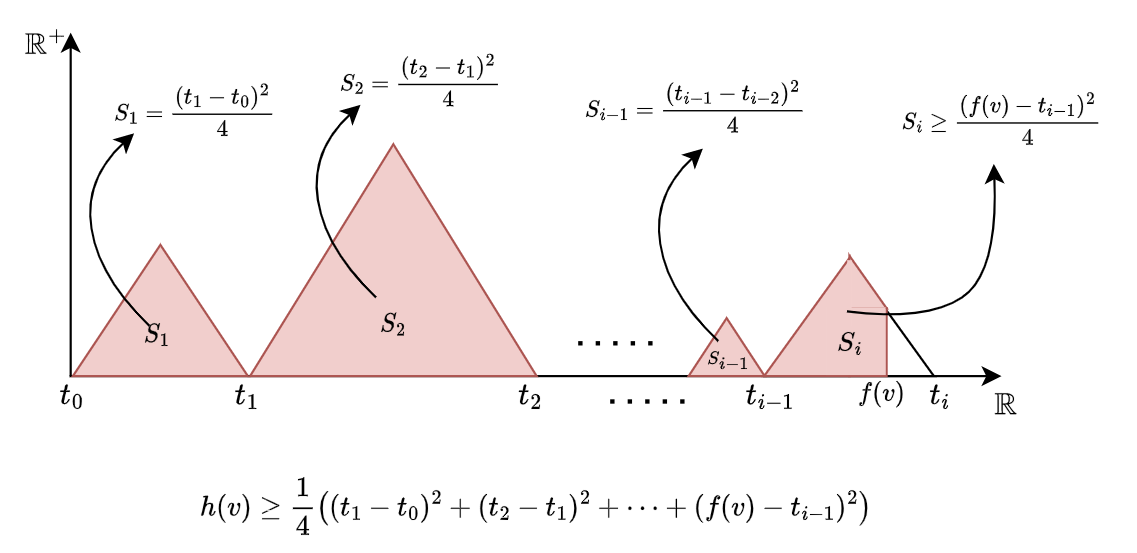
\includegraphics[width=0.5\textwidth]{images/h_lower_bound.png}
    \caption{Illustration of $\mu(x)$ and $h(x)$.}
\end{figure}
    \textbf{Step 1}: \textit{Lower Bounding the Denominator.} We begin by establishing the lower bound
    \begin{equation}
        h(v) \geq \frac{1}{8k}f(v)^2.
    \end{equation}
    Suppose $f(v) \in [t_i,t_{i+1}]$. Then,
    \begin{align*}
        h(v) &= \sum_{j=0}^{i-1}\int_{t_j}^{t_{j+1}}\mu(x)dx + \int_{t_i}^{f(v)}\mu(x)dx\\
        &= \sum_{j=0}^{i-1}\frac{1}{4}(t_{j-1} - t_j)^2 + \int_{t_j}^{f(v)}\mu(x)dx\\
        &\geq \sum_{j=0}^{i-1}\frac{1}{4}(t_{j-1}-t_j)^2 + \frac{1}{4}(f(v) - t_i)^2.
    \end{align*}
    Next, we relate the above lower bound to $f(v)^2$ via the following computation
    $$f^2(v) = \left(\sum_{j=0}^{i-1}(t_{j+1}-t_j) + f(v) - t_i\right)^2 \leq 2k\left(\sum_{j=0}^{i-1}(t_{j+1}-t_j)^2 + (f(v)-t_i)^2\right),$$
    where the inequality follows from the Cauchy-Schwartz inequality. Thus we derived our desired result.

    \textbf{Step 2}: \textit{Upper Bounding the Numerator.} We begin by investigating the smoothness of $h$. WLOG assume $f(u) \leq f(v)$. By definition, for $x \in [f(u),f(v)]$, $\mu(x) \leq \min\{\abs{x-g(u)},\abs{x-g(v)}\}$. Hence we can write
    \begin{align*}
        \mu(x) &\leq \frac{\abs{x-g(u)} + \abs{x-g(v)}}{2}\\
        &\stackrel{\text{(a)}}{\leq} \frac{1}{2}\left(\abs{x - f(u)} + \abs{f(u) - g(u)} + \abs{x-f(v)} + \abs{f(v) - g(v)}\right)\\
        &= \frac{1}{2}\left(\abs{f(u) - f(v)} + \abs{f(u) - g(u)} + \abs{f(v) - g(v)}\right),
    \end{align*}
    where (a) follows from the triangle inequality. Consequently,
    $$h(v) - h(u) = \int_{f(u)}^{f(v)}\mu(x)dx \leq \frac{1}{2}\abs{f(u) - f(v)}\left(\abs{f(u) - f(v)} + \abs{f(u) - g(u)} + \abs{f(v) - g(v)}\right).$$
    Next, we upper bound the numerator,
    \begin{align*}
        \sum_{\{u,v\} \in E}w(u,v)\abs{h(u) - h(v)} &\leq \sum_{\{u,v\} \in E}\frac{1}{2}w(u,v)\abs{f(u) - f(v)}\left(\abs{f(u) - f(v)} + \abs{f(u) - g(u)} + \abs{f(v) - g(v)}\right)\\
        &\stackrel{\text{(a)}}{\leq} \sum_{\{u,v\} \in E}\frac{1}{2}w(u,v)\abs{f(u) - f(v)}^2 \\
        &+ \frac{1}{2}\sqrt{\sum_{\{u,v\} \in E}w(u,v)\abs{f(u) - f(v)}^2}\sqrt{\sum_{\{u,v\} \in E}w(u,v)\left(\abs{f(u) - g(u)}^2 + \abs{f(v) - g(v)}^2\right)}\\
        &\stackrel{\text{(b)}}{=} \frac{1}{2}\calR(f) + \frac{1}{2}\sqrt{2\calR(f)}\norm{f-g}_w,
    \end{align*}
    where (a) follows from the Cauchy-Schwartz inequality, and (b) holds since $\norm{f}_w = 1$.

    Combining steps 1 and 2, we get
    \begin{equation}
        \frac{\sum_{\{u,v\} \in E}w(u,v)\abs{h(u) - h(v)}}{\sum_v w(v)h(v)} \leq 4k\calR(f) + 4k\sqrt{2\calR(f)}\norm{f-g}_w.
    \end{equation}
    Invoking Lemma \ref{lem_phi_h} and using $\phi(h) = \phi(f)$ completes the proof.
\end{proof}

With Proposition \ref{prop:phi_f} in hand, we are ready to present the proof of Theorem \ref{thm:improved_cheeger}.

\begin{proofof}{of Theorem \ref{thm:improved_cheeger}}
    Choose $f$ from Corollary \ref{cor:good_f}, and let $g$ be the $2k+1$-step approximation from Lemma \ref{lem:approx} such that $\norm{f-g}_w \leq 2\sqrt{\tfrac{\calR(f)}{\lambda_k}}$. Applying Proposition \ref{prop:phi_f} and using $\calR(f) \leq \lambda_2$ we have
    $$\phi(f) \leq 4k\lambda_2 + 8\sqrt{2}k\frac{\lambda_2}{\sqrt{\lambda_k}} \leq 12\sqrt{2}k\frac{\lambda_2}{\sqrt{\lambda_k}},$$
    where the second inequality holds since $\lambda_k \leq 2$. Finally, by definition $\phi(G) \leq \phi(f)$, which completes the proof of the theorem.
\end{proofof}




\end{document}



